% ============================================================
%  CHAPITRE 4 — ÉVALUATION EXPÉRIMENTALE ET RÉSULTATS
% ============================================================
\chapter{Évaluation Expérimentale et Résultats}
\label{chap:evaluation}

\section{Introduction}

Ce chapitre évalue objectivement les performances du modèle développé au chapitre~\ref{chap:modele}, afin de vérifier sa capacité à identifier des zones d'atterrissage sécurisées et à détecter les obstacles critiques sur des données jamais vues durant l'entraînement. L'évaluation combine des métriques quantitatives et une inspection visuelle des résultats produits lors de l'inférence. Pour cela, nous définissons d'abord les métriques mathématiques retenues pour mesurer cette performance.

\section{Métriques d'évaluation}
\label{sec:metriques}

Pour évaluer de manière rigoureuse la qualité de la segmentation binaire (classes SAFE et UNSAFE) réalisée par notre modèle, nous nous basons sur la matrice de confusion en pixel. En notant $TP$ les vrais positifs (pixels d'obstacles ou praticables correctement identifiés), $TN$ les vrais négatifs, $FP$ les faux positifs (pixels incorrectement prédits comme appartenant à la classe), et $FN$ les faux négatifs (pixels de la classe manqués par la prédiction), nous définissons les métriques suivantes :

\subsection{Intersection over Union (IoU)}
L'Intersection over Union (\textit{IoU}), ou indice de Jaccard, mesure le taux de recouvrement spatial entre le masque de prédiction sémantique et le masque de vérité terrain. Dans le contexte de l'atterrissage, elle quantifie la précision globale de la délimitation géographique des zones sûres :
\begin{equation}
  \text{IoU} = \frac{TP}{TP + FP + FN}
\end{equation}

\subsection{Dice Score}
Le \textit{Dice Score} (ou coefficient de Sørensen-Dice) mesure la similitude globale entre deux échantillons. Elle est mathématiquement équivalente au F1-Score au niveau des pixels et se montre particulièrement sensible aux correspondances locales, ce qui la rend directement cohérente avec la fonction de coût hybride utilisée lors de l'entraînement :
\begin{equation}
  \text{Dice Score} = \frac{2 \cdot TP}{2 \cdot TP + FP + FN}
\end{equation}

\subsection{Précision (Precision)}
La \textit{Précision} évalue la proportion de pixels correctement classés comme praticables (SAFE) parmi tous les pixels prédits comme tels. Dans notre application, elle mesure la fiabilité des zones déclarées sûres, garantissant qu'aucune zone dangereuse (contenant un obstacle) ne soit classée par erreur comme zone d'atterrissage :
\begin{equation}
  \text{Precision} = \frac{TP}{TP + FP}
\end{equation}

\subsection{Rappel (Recall)}
Le \textit{Rappel} (ou sensibilité) mesure la proportion d'obstacles ou de surfaces praticables correctement identifiés par rapport à leur présence réelle dans la vérité terrain. Dans notre contexte, il quantifie la capacité du modèle à détecter tous les obstacles réels sans en omettre, ce qui est absolument critique pour éviter des collisions dramatiques lors de l'évitement bas niveau :
\begin{equation}
  \text{Recall} = \frac{TP}{TP + FN}
\end{equation}

\subsection{F1-Score}
Le \textit{F1-Score} correspond à la moyenne harmonique de la Précision et du Rappel. Il offre un indicateur de performance synthétique et équilibré, particulièrement pertinent en présence de classes déséquilibrées (par exemple, lorsque les obstacles n'occupent qu'une faible fraction de la scène capturée) :
\begin{equation}
  \text{F1-Score} = 2 \cdot \frac{\text{Precision} \cdot \text{Recall}}{\text{Precision} + \text{Recall}}
\end{equation}

Ces définitions étant posées, les objectifs et seuils d'interprétation pour la validation finale du système d'atterrissage sont résumés dans la Table~\ref{tab:metriques}.

\begin{table}[!ht]
  \centering
  \caption{Métriques d'évaluation retenues et leur interprétation.}
  \label{tab:metriques}
  \renewcommand{\arraystretch}{1.4}
  \begin{tabularx}{0.95\textwidth}{
    >{\bfseries\color{ENIADBlue}}l
    >{\centering\arraybackslash}X
    >{\arraybackslash}X
  }
    \toprule
    \rowcolor{ENIADBlue!12}
    \textbf{Métrique} & \textbf{Objectif} & \textbf{Interprétation} \\
    \midrule
    IoU & Recouvrement spatial & $>$0.85 : excellent · 0.70--0.85 : bon · 0.50--0.70 : acceptable \\
    \rowcolor{ENIADLightBlue!20}
    Dice Score & Similitude globale & Cohérent avec la fonction de coût \\
    Precision & Éviter les fausses zones sûres & Critique pour la sécurité finale \\
    \rowcolor{ENIADLightBlue!20}
    Recall & Détecter tous les obstacles & Un obstacle manqué est plus grave qu'une fausse alerte \\
    F1-Score & Équilibre Precision/Recall & $>$0.85 : excellent · 0.70--0.85 : bon · 0.50--0.70 : acceptable \\
    \bottomrule
  \end{tabularx}
\end{table}

Ces définitions posées, nous analysons dans la section suivante les courbes et les performances quantitatives enregistrées lors des époques d'apprentissage.

\section{Résultats d'entraînement}
\label{sec:resultats-entrainement}

Le modèle a été entraîné sur un maximum de 150 époques, avec arrêt anticipé (patience = 15) déclenché à l'époque 128. Le meilleur modèle, retenu selon la perte de validation minimale, a été obtenu à l'\textbf{époque 113} :

\begin{table}[!ht]
  \centering
  \caption{Résultats quantitatifs du meilleur modèle (époque 113).}
  \label{tab:resultats}
  \renewcommand{\arraystretch}{1.4}
  \begin{tabularx}{0.75\textwidth}{
    >{\bfseries\color{ENIADBlue}}l
    >{\centering\arraybackslash}X
    >{\centering\arraybackslash}X
  }
    \toprule
    \rowcolor{ENIADBlue!12}
    \textbf{Indicateur} & \textbf{Entraînement} & \textbf{Validation} \\
    \midrule
    Loss & 0.1599 & 0.1262 \\
    \rowcolor{ENIADLightBlue!20}
    IoU & 0.8542 & \textbf{0.8803} \\
    Dice Score & 0.9179 & \textbf{0.9349} \\
    \rowcolor{ENIADLightBlue!20}
    Precision & 0.9135 & \textbf{0.9305} \\
    Recall & 0.9223 & \textbf{0.9393} \\
    \rowcolor{ENIADLightBlue!20}
    F1-Score & 0.9179 & \textbf{0.9349} \\
    \bottomrule
  \end{tabularx}
\end{table}

L'évaluation détaillée du meilleur modèle met en évidence de très fortes performances de généralisation. Le rappel (\textit{Recall}) élevé de \textbf{0.9393} en validation confirme que le réseau parvient à isoler et à identifier la quasi-totalité des obstacles et des zones dangereuses de la scène aérienne, limitant au maximum le risque d'une omission de danger qui s'avérerait fatale pour l'aéronef. Parallèlement, la précision (\textit{Precision}) solide de \textbf{0.9305} atteste de la fiabilité des zones classées comme praticables (SAFE), minimisant le risque de fausses alarmes de sécurité. Le F1-Score global de \textbf{0.9349} (équivalent au Dice Score au niveau des pixels) résume de manière équilibrée cette synergie entre précision de guidage et évitement d'obstacles. Ces valeurs représentent des estimations cohérentes à valider lors d'analyses approfondies des logs.

Les courbes montrent une décroissance rapide de la perte durant les 15 à 20 premières époques (favorisée par le transfert d'apprentissage via l'encodeur EfficientNet-B0 pré-entraîné), suivie d'une phase de stabilisation progressive menant à l'obtention du meilleur modèle à l'époque 113. L'ensemble des métriques d'évaluation sémantique suit cette dynamique d'amélioration : l'IoU, le Dice Score et le F1-Score progressent de manière synchrone pour atteindre respectivement des valeurs de validation finales de \textbf{0.880}, \textbf{0.935} et \textbf{0.935}. En parallèle, la Precision (détection fiable sans fausses alarmes) et le Recall (couverture complète des obstacles) augmentent de façon stable, convergeant vers des scores de validation élevés de \textbf{0.931} et \textbf{0.939} (figure~\ref{fig:training-curves}).

\begin{figure}[!ht]
  \centering
  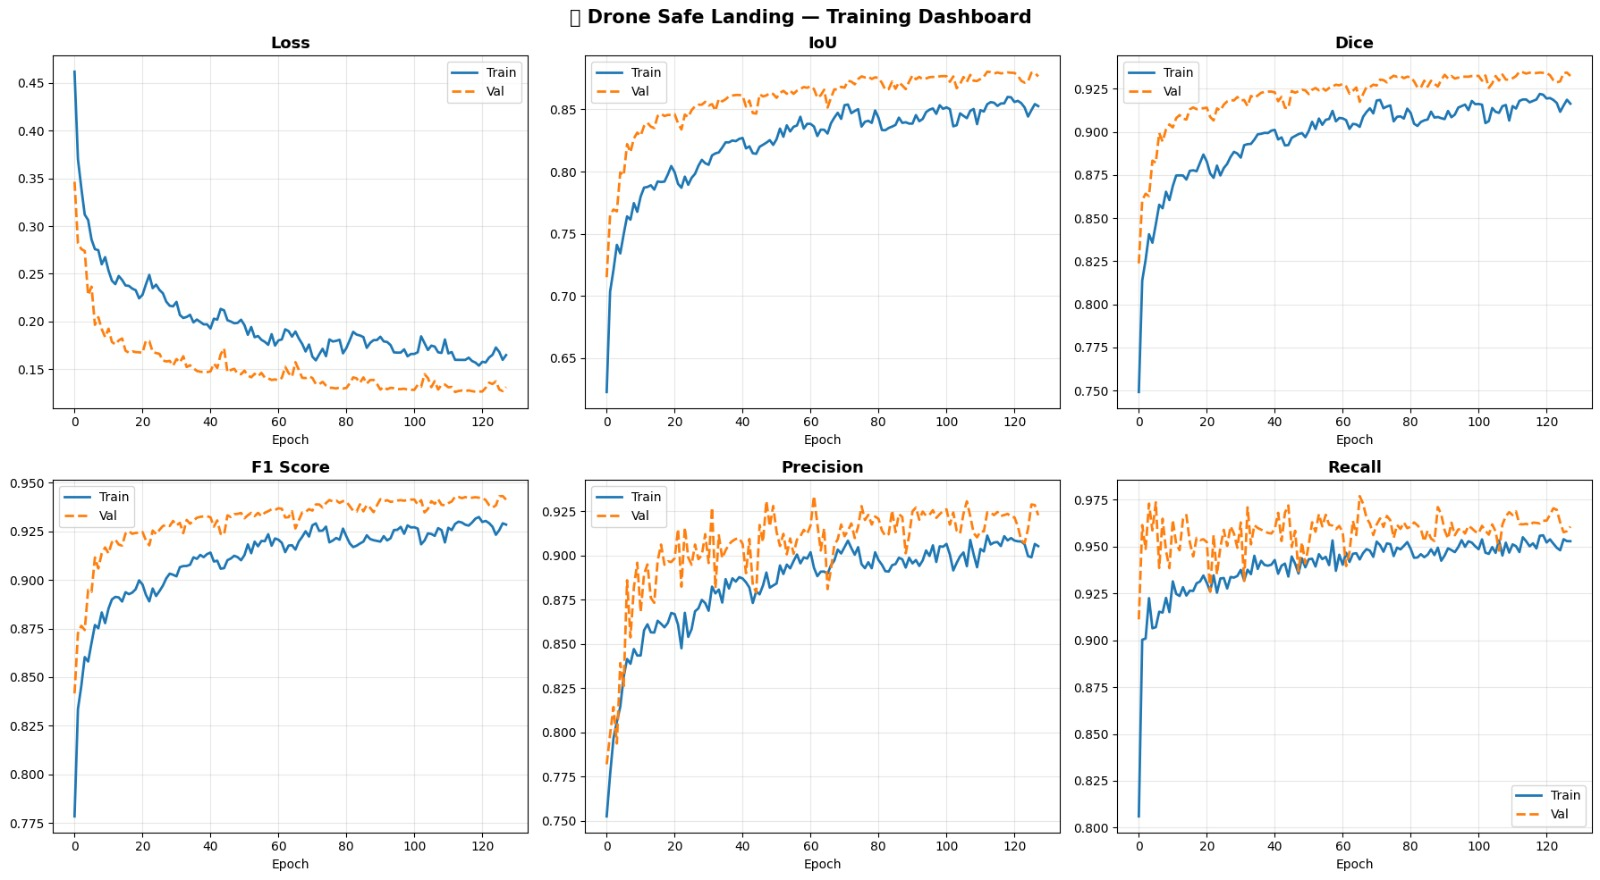
\includegraphics[width=0.75\textwidth,keepaspectratio]{diagramme.jpeg}
  \caption{Courbes d'évolution de la perte (Loss), de l'IoU, du Dice Score, du F1-Score, de la Precision et du Recall en entraînement et validation.}
  \label{fig:training-curves}
\end{figure}

Les journaux d'entraînement (logs console) confirment le bon déroulement du processus, avec la sauvegarde automatique des checkpoints dès qu'une amélioration de la perte de validation est détectée (figure~\ref{fig:training-logs}). Cet extrait montre en particulier les métriques intermédiaires obtenues entre les époques 98 et 101, illustrant la phase de stabilisation progressive. L'entraînement s'est ensuite poursuivi au-delà de cette phase jusqu'à atteindre les performances optimales du meilleur modèle sauvegardé à l'époque 113, avant le déclenchement final de l'arrêt anticipé (Early Stopping) après stabilisation à l'époque 128.

\begin{figure}[!ht]
  \centering
  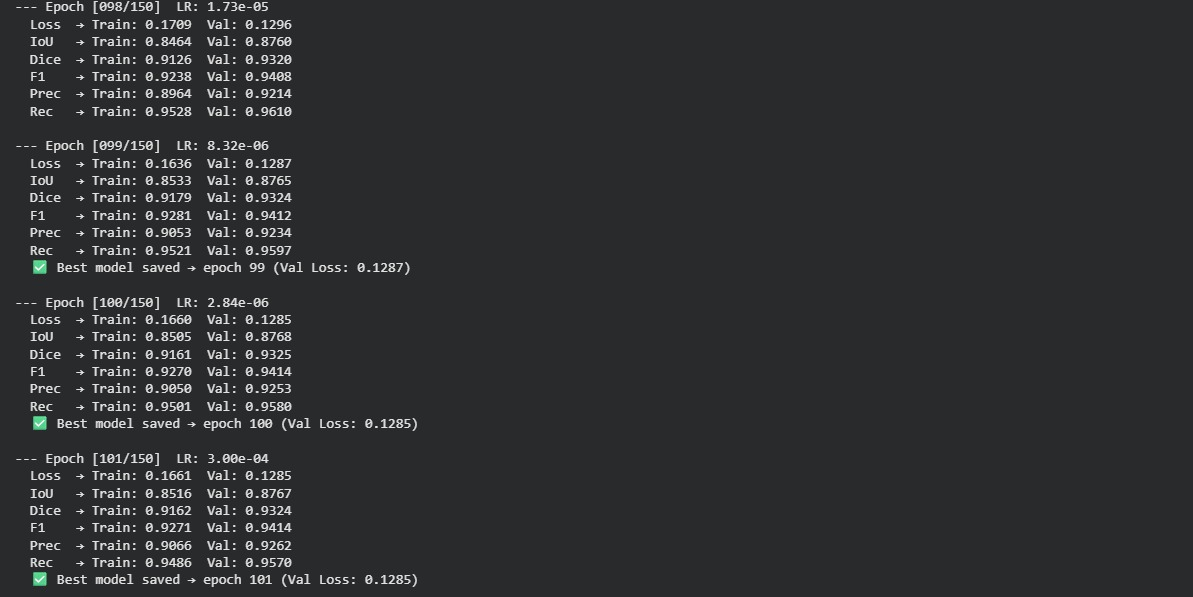
\includegraphics[width=0.65\textwidth,keepaspectratio]{train_Epochs.jpeg}
  \caption{Extrait des journaux d'entraînement (logs console) montrant l'évolution des métriques (Loss, IoU, Dice, F1, Precision, Recall) entre les époques 98 et 101, avec sauvegarde automatique du meilleur modèle.}
  \label{fig:training-logs}
\end{figure}

\textbf{\textcolor{red}{Note :}} Les courbes de validation restent globalement proches des courbes d'entraînement tout au long du processus — la perte de validation est même légèrement inférieure à la perte d'entraînement sur les dernières époques —, ce qui n'indique pas de surapprentissage marqué. La Data Augmentation et la régularisation (Weight Decay) semblent avoir rempli leur rôle.

Au-delà des scores globaux, la validation du système repose sur une inspection visuelle directe des prédictions du modèle sur des scènes réelles, présentée ci-après.

\section{Résultats visuels}
\label{sec:resultats-visuels}

L'inspection qualitative sur un échantillon varié de scènes de test (figure~\ref{fig:predictions-comparison}) confirme la précision spatiale du modèle. Les quatre exemples présentés illustrent la capacité du réseau à segmenter correctement les surfaces d'atterrissage praticables tout en isolant les piétons, véhicules et autres obstacles critiques, avec des scores d'intersection sur union (IoU) individuels élevés.

\begin{figure}[!hb]
  \centering
  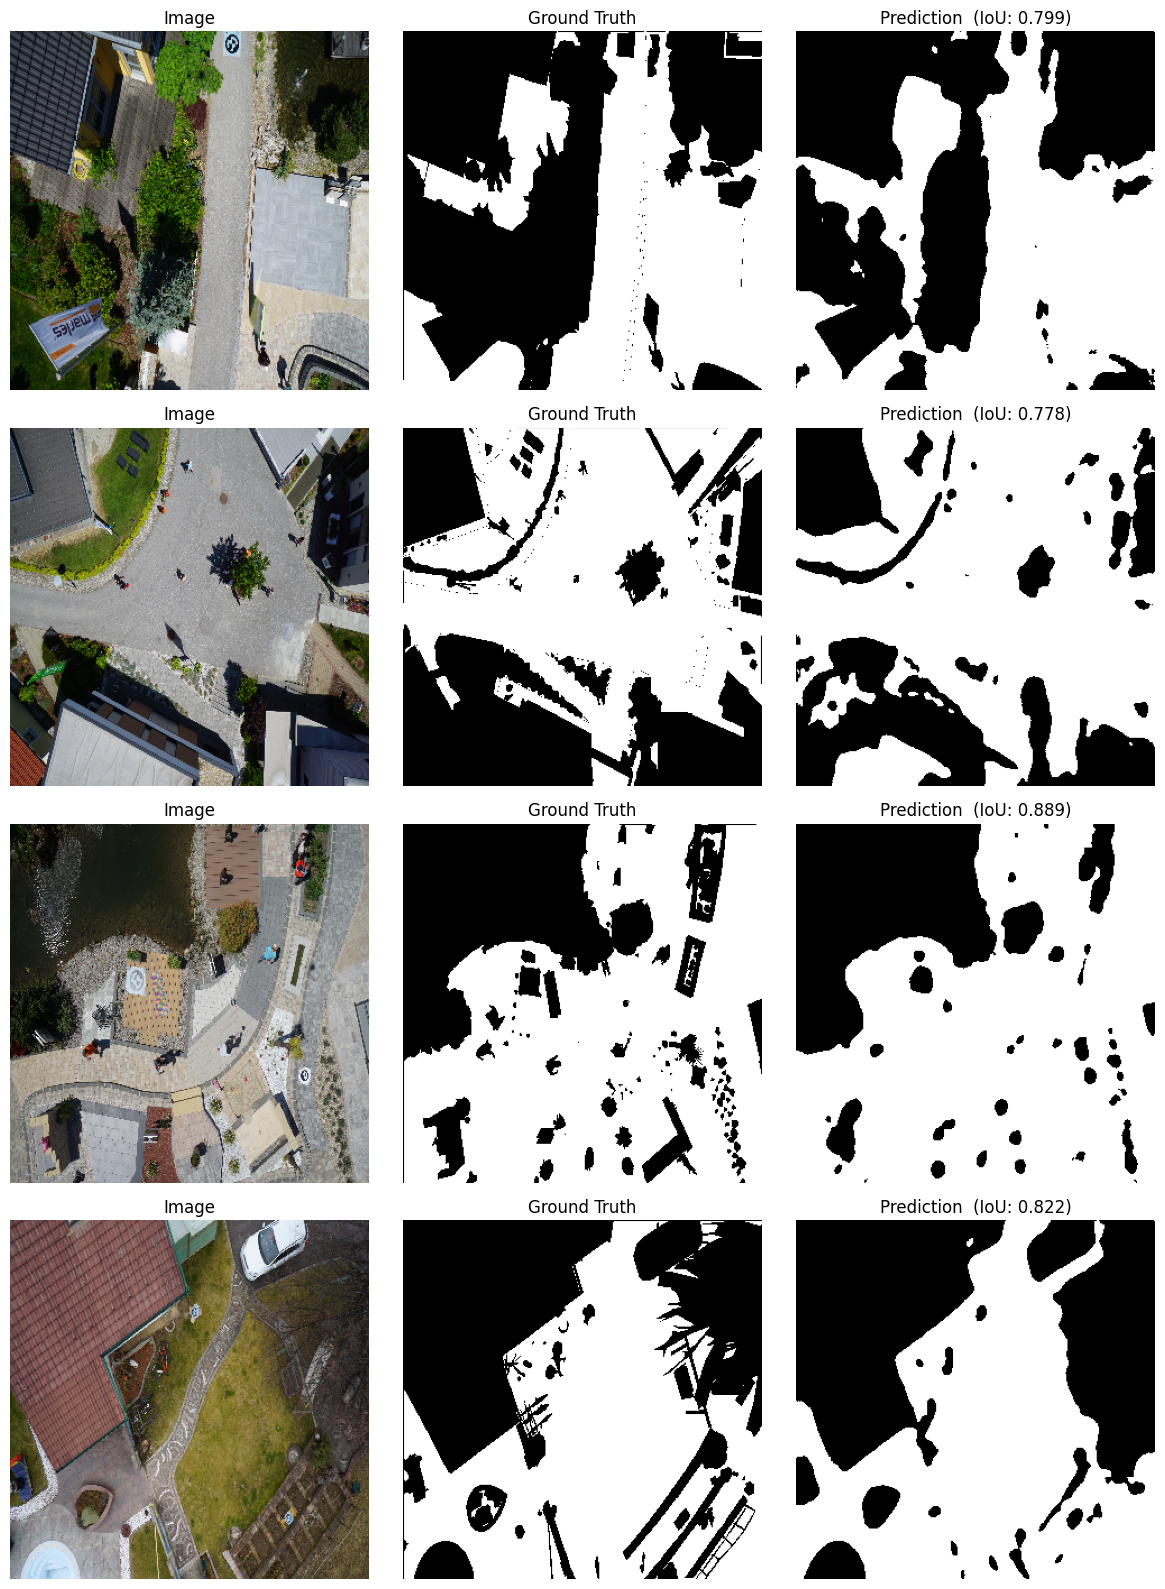
\includegraphics[width=0.7\textwidth,keepaspectratio]{slide14_resultats_visuels.png}
  \caption{Comparaison qualitative sur le dataset de test pour quatre exemples caractéristiques : image d'entrée, vérité terrain (Ground Truth) et masque de prédiction sémantique avec l'indice de Jaccard (IoU) obtenu pour chaque scène.}
  \label{fig:predictions-comparison}
\end{figure}

Ce comportement illustre le fonctionnement attendu du pipeline de décision : la conversion du masque sémantique en carte binaire exploitable identifie correctement les obstacles ponctuels (personnes, objets) tout en conservant de larges surfaces continues pour l'atterrissage.

Afin de situer la performance de notre modèle sémantique par rapport aux standards actuels, nous le comparons avec les architectures de référence de la littérature.

\section{Comparaison avec les architectures de la littérature}
\label{sec:comparaison}

Le choix de l'architecture U-Net + EfficientNet-B0 a été justifié au chapitre~\ref{chap:dataset} par une comparaison qualitative avec les approches les plus utilisées en segmentation sémantique. FCN offre un coût de calcul faible mais une reconstruction des détails plus limitée ; DeepLabV3 et SegFormer atteignent une précision potentiellement supérieure au prix d'un coût mémoire et d'un temps d'inférence incompatibles avec les contraintes Edge AI.

Les résultats obtenus (IoU 0.8803, Dice 0.9349) confirment qu'une architecture plus légère, correctement optimisée, peut atteindre un niveau de performance élevé tout en restant compatible avec un déploiement embarqué. Pour finaliser cette évaluation, il convient de dresser un bilan critique des forces de notre approche ainsi que des limites qui tracent les perspectives futures.

\section{Discussion, forces et limites}
\label{sec:discussion}

Les résultats obtenus valident l'approche retenue : un IoU de validation de \textbf{0.8803}, un Dice Score de \textbf{0.9349}, une précision de \textbf{0.9305}, un rappel de \textbf{0.9393} et un F1-Score global de \textbf{0.9349}. Ces niveaux de performance, classés comme \textit{excellents} selon les seuils établis, démontrent la robustesse du réseau tant pour la détection fiable des zones praticables que pour la non-omission d'obstacles critiques, le tout avec une convergence stable et sans surapprentissage marqué.

Ces résultats doivent néanmoins être interprétés avec les réserves suivantes :
\begin{itemize}[leftmargin=1.8em, itemsep=4pt]
  \item[\textcolor{ENIADOrange}{\ding{118}}] Le dataset reste limité (400 images), ce qui restreint la diversité des scènes réellement couvertes ;
  \item[\textcolor{ENIADOrange}{\ding{118}}] Les métriques sont mesurées hors ligne, et non lors d'une exécution embarquée en conditions réelles ;
  \item[\textcolor{ENIADOrange}{\ding{118}}] La comparaison avec d'autres architectures reste théorique faute de benchmark empirique direct.
\end{itemize}

\vspace{1.5em}
\textbf{Conclusion}

En conclusion, ce quatrième et dernier chapitre a permis de valider expérimentalement les performances du système développé en obtenant des scores élevés en validation (IoU de 0.8803 et Dice Score de 0.9349) et en confirmant qualitativement la fiabilité de la Distance Transform. Les discussions critiques ont également tracé la voie pour de futures améliorations matérielles et de déploiement réel. Ce bilan expérimental venant clore notre étude technique, la conclusion générale suivante synthétisera l'ensemble de nos contributions académiques et ouvrira sur les perspectives industrielles à long terme de ce projet.
\clearpage
